%
% CMPT 300: Operating Systems I - A Course Overview
% Section: Memory Management
%
% Author: Jeffrey Leung
%

\section{Memory Management}
	\label{sec:memory-management}
\begin{easylist}

& Code location can be absolute if memory location is known during compile time, or relocatable otherwise

& \textbf{Physical address:} Location in physical memory accessed by the memory unit
& \textbf{Logical/virtual address:} CPU-managed location in memory 
	&& Different from physical address if addresses are bound during execution
	&& \textbf{Memory Management Unit (MMU):} Hardware component which maps virtual addresses to physical addresses during runtime
		&&& Ensures separation and protection of memory areas
		&&& Basic components: Base and limit register

\end{easylist}
\subsection{Contiguous Allocation}
	\label{subsec:memory-management:contiguous-allocation}
\begin{easylist}

& Allocation algorithms:
	&& \textbf{First-fit algorithm:} Allocating memory in the first available sufficiently-sized hole
	&& \textbf{Best-fit algorithm:} Allocating memory in the smallest sufficiently-sized hole to create the smallest possible remaining hole
		&&& Requires searching the entire memory space
	&& \textbf{Worst-fit algorithm:} Allocating memory in the largest sufficiently-sized hole to create the largest possible remaining hole
		&&& Requires searching the entire memory space

& \textbf{External fragmentation:} Situation where the memory space exists to fulfill a request but it is not contiguous
	&& \textbf{Memory compaction:} Method to solve external fragmentation which places all free memory together
		&&& Only possible if addresses are bound during execution

\end{easylist}
\subsection{Paging}
	\label{subsec:memory-management:paging}
\begin{easylist}

& \textbf{Page:} Fixed-size, contiguous logical memory unit for non-contiguous memory allocation
	&& \textbf{Frame:} Fixed-size, contiguous physical memory unit for non-contiguous memory allocation
		&&& Associated 1:1 with each page

& Components of addresses:
	&& \textbf{Page number:} Component which contains the base address of a page in physical memory
	&& \textbf{Page offset:} Component which contains an offset of the base address sent to the MMU
	&& For $m, n$ where the address space is $2^m$ and the page size has $2^n$ entries, the number of pages is $\frac{2^m}{2^n} = 2^{m-n}$, the address has $m$ bits, the page number has $m-n$ bits, and the page offset has $n$ bits
	&& Size: Power of 2 (so that the page number and offset can be easily navigated)

& \textbf{Page table:} Set of translations from logical memory to physical memory
	&& Allows partitioning of physical memory and linkage with virtual memory in arbitrary ordering
	&& Specific to each process
	&& Located through the page table base register
	&& Requires two memory accesses (one for page table, one for instruction)
	&& Includes protection bits to specify if a page is read-only/read-write/execute-only, or if a page is valid/invalid access for the process
	&& Diagram: See figure~\ref{fig:paging:page-table-1}

	\begin{figure}[!htb]
		\centering
		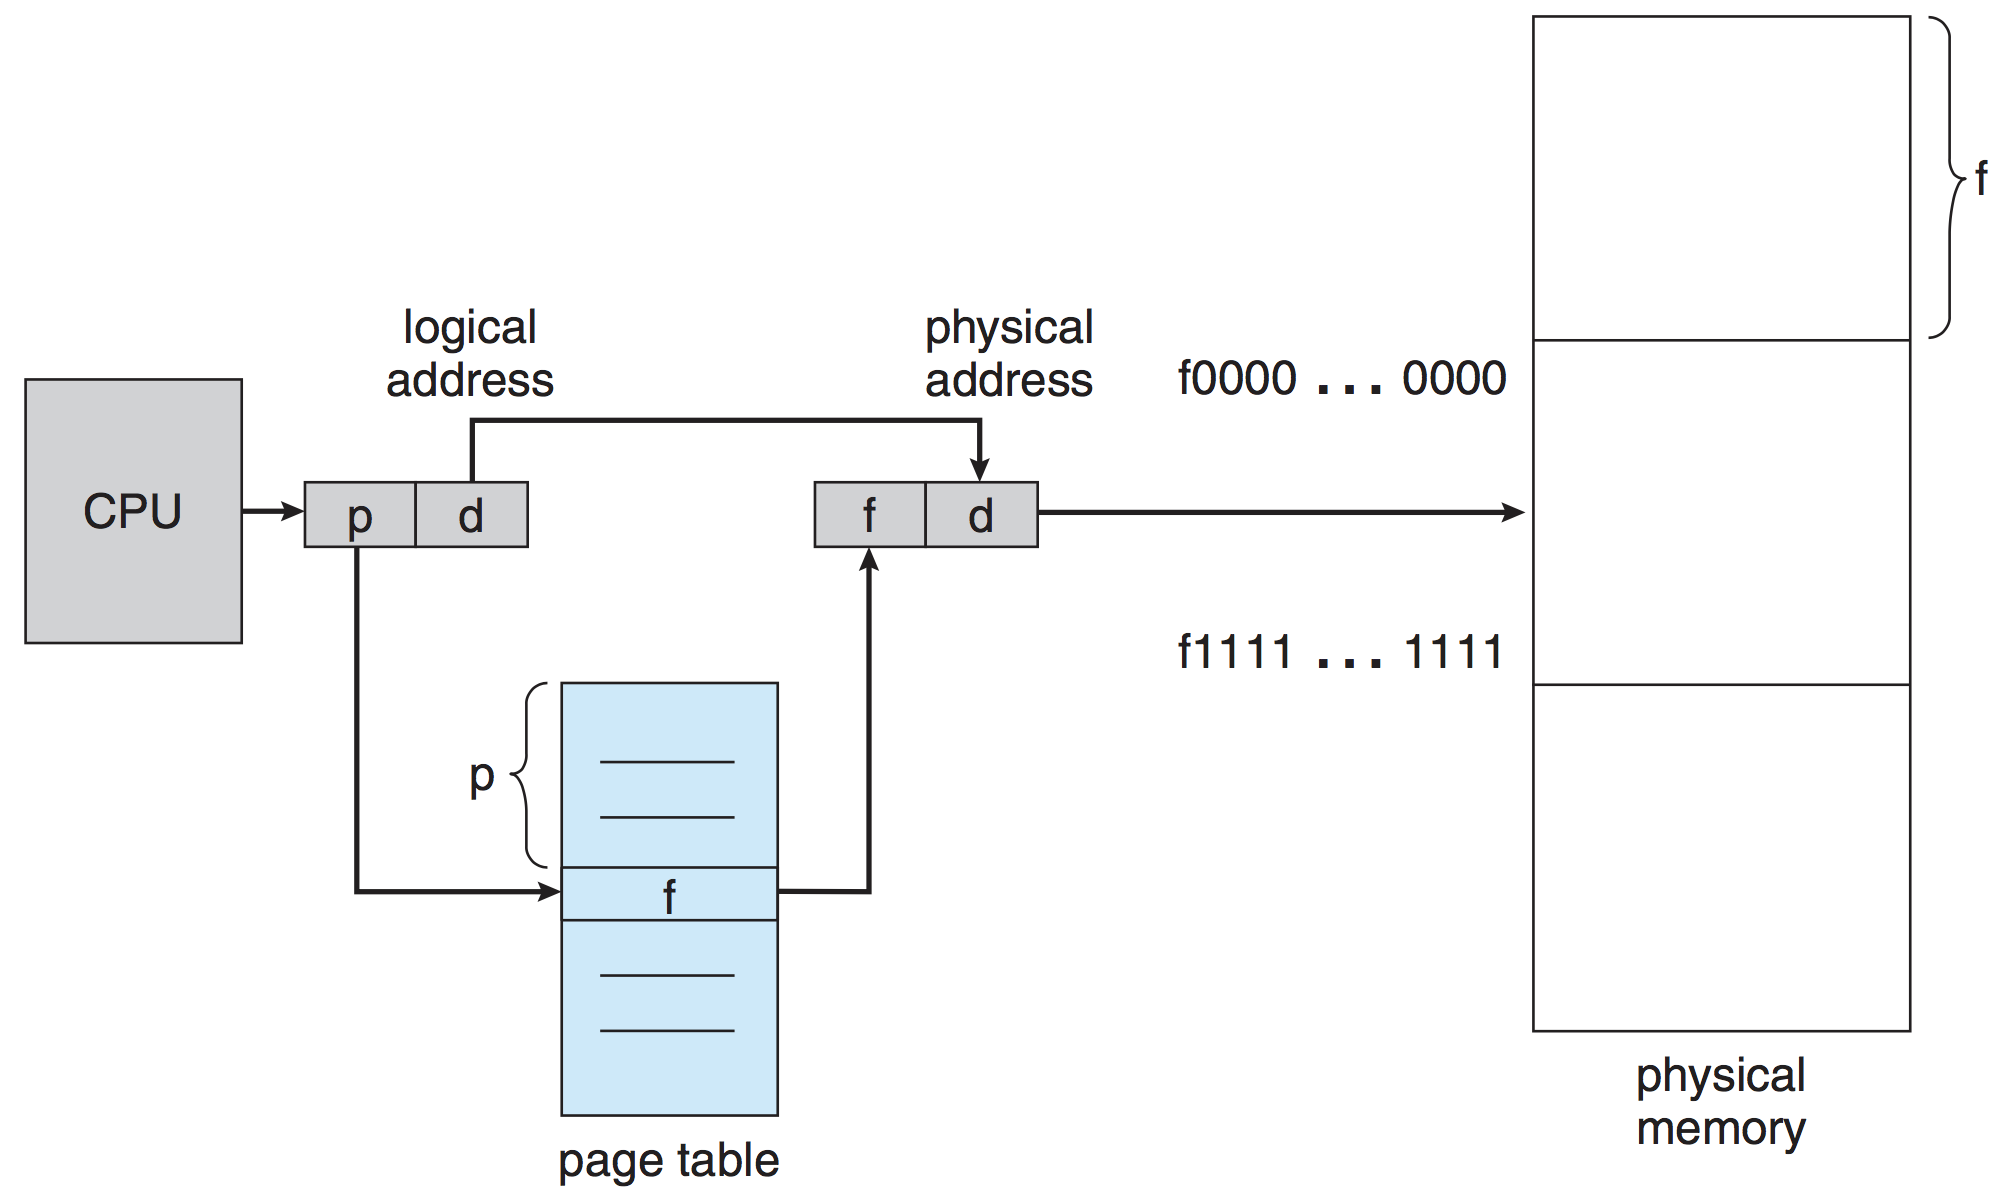
\includegraphics[width=0.7\textwidth]{page-table-1}
		\caption{Diagram of a Page Table}
		\label{fig:paging:page-table-1}
	\end{figure}
	
	&& Page table address translation process:
	\end{easylist}
	\begin{align*}
		\textrm{Let } s &= \textrm{ page/frame size }\\
		\textrm{Let } p &= \textrm{ page number }\\
		\textrm{Let } d &= \textrm{ offset}, 0 \leq d < s \\
		\textrm{Logical address } &= p \times s + d \\
		\textrm{Let } f &= \textrm{ frame number translated from } p \textrm{ using page table } \\
		\textrm{Physical address } &= f \times s  + d
	\end{align*}
	\begin{easylist}
	
		&&& Example:
		\end{easylist}
		\begin{align*}
			\textrm{Page/frame size } s &= 4 \textrm{ bytes} \\
			\textrm{Page table: }
			& 0 \rightarrow 5 \\
			& 1 \rightarrow 6 \\
			& 2 \rightarrow 1 \\
			& 3 \rightarrow 2 \\
			\textrm{Logical address }
			&= 0 \\
			&= p \times s + d \\
			&= 0 \times 4 + 0 \\
			f_{p=0} &= 5 \\
			\textrm{Physical address } &= f \times s + d \\
			&= 5 \times 4 + 0 \\
			&= 20
		\end{align*}
		\begin{easylist}
	
		&&& Example:
		\end{easylist}
		\begin{align*}
			\textrm{Page/frame size } s &= 4 \textrm{ bytes} \\
			\textrm{Page table: }
			& 0 \rightarrow 5 \\
			& 1 \rightarrow 6 \\
			& 2 \rightarrow 1 \\
			& 3 \rightarrow 2 \\
			\textrm{Logical address }
			&= 13 \\
			&= p \times s + d \\
			&= 3 \times 4 + 1 \\
			f_{p=3} &= 2 \\
			\textrm{Physical address } &= f \times s + d \\
			&= 2 \times 4 + 1 \\
			&= 9
		\end{align*}
		\begin{easylist}

& \textbf{Translation Look-aside Buffer (TLB):} Fast-lookup associative memory structure which stores recently used page table entries
	&& \textbf{Address Space Identifier:} Component of a TLB entry containing a process ID for protection
	&& Common across processes
	&& If the page is not found, the page table is used and the entry is added to the TLB
		&&& Some TLB entries are fixed and cannot be replaced (e.g. kernel codes)
	&& Diagram: See figure~\ref{fig:paging:page-table-2-tlb}

	\begin{figure}[!htb]
		\centering
		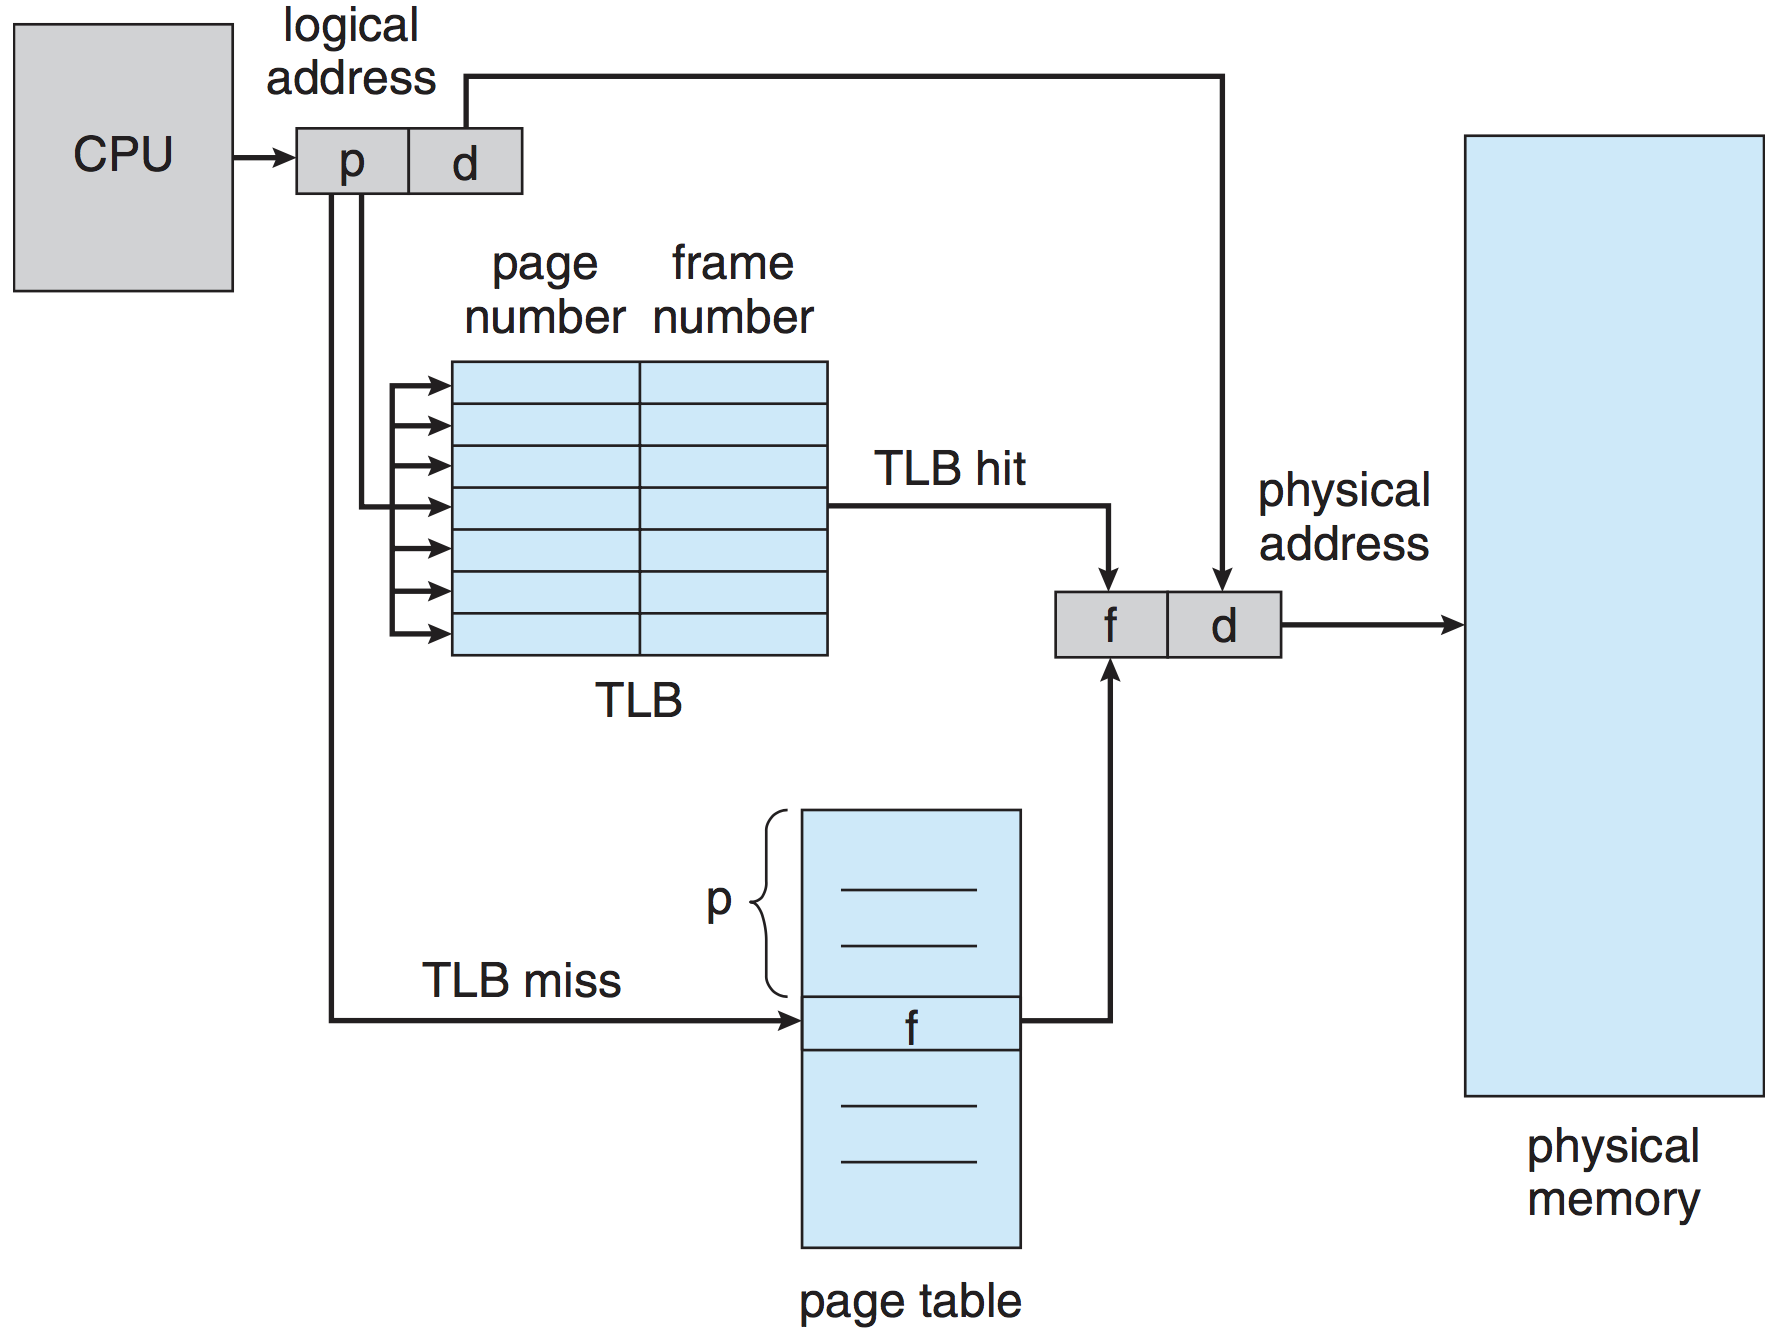
\includegraphics[width=0.7\textwidth]{page-table-2-tlb}
		\caption{Diagram of a TLB}
		\label{fig:paging:page-table-2-tlb}
	\end{figure}

& \textbf{Effective Access Time:} Amortized time for TLB lookup and page table access
	&& TLB hit ratio is proportional to the effective access time between the time for 1 memory access and the time for 2 memory accesses
	&& Equation:
	\end{easylist}
	\begin{align*}
		\textrm{ Let } t_m &= \textrm{ memory access time} \\
		\textrm{ Let } \varepsilon &= \textrm{ TLB lookup time (significantly less than } t_m \textrm{)} \\
		\textrm{ Let } \alpha &= \textrm{ TLB hit ratio (percentage of times page found in TLB)} \\
		\textrm{Effective Access Time }
		&= \textrm{ Time for TLB hit } \times \textrm{ TLB hit percentage } + \\
		& \textrm{ Time for TLB miss } \times \textrm{ TLB miss percentage } \\
		&= (\varepsilon + t_m) \times \alpha + (\varepsilon + 2 \times t_m) \times (1 - \alpha) \\
		&= \varepsilon + t_m \times (2 - \alpha) \\
	\end{align*}
	\begin{easylist}
	
		&&& Example:
		\end{easylist}
		\begin{align*}
			\textrm{ Let } t_m &= 100 \textrm{ ns} \\
			\textrm{ Let } \varepsilon &= 0 \\
			\textrm{ Let } \alpha &= 0.8 \\
			\textrm{Effective Access Time }
			&= \varepsilon + t_m \times (2 - \alpha) \\
			&= 100 \textrm{ ns } \times (2 - 0.8) \\
			&= 120 \textrm{ ns} \\
			\textrm{Slowdown } &= \frac{100 \textrm{ ns}}{120 \textrm{ ns}} - 1 = 20\% \\
		\end{align*}
		\begin{easylist}
	
		&&& Example:
		\end{easylist}
		\begin{align*}
			\textrm{ Let } t_m &= 100 \textrm{ ns} \\
			\textrm{ Let } \varepsilon &= 0 \\
			\textrm{ Let } \alpha &= 0.99 \\
			\textrm{Effective Access Time }
			&= \varepsilon + t_m \times (2 - \alpha) \\
			&= 100 \textrm{ ns } \times (2 - 0.99) \\
			&= 101 \textrm{ ns} \\
			\textrm{Slowdown } &= \frac{100 \textrm{ ns}}{101 \textrm{ ns}} - 1 = 1\% \\
		\end{align*}
		\begin{easylist}

& \textbf{Reentrant code:} Read-only code shared among multiple processes
	&& Must appear in the same location in the logical address spaces due to processes sharing a TLB

& Page table structural alternatives:
	&& Page table requires contiguous memory or the page table will need to be paged itself
	&& For an address space of $32$ bits and a page size of $4$ KB ($2^{12}$ bytes), a process could have $2^{32-12} = 2^{20}$ pages; for a page table with entries of $4$ bytes, the size of a page table for each process could be $2^{20} \times 4 = 2^{22} $ bytes $ = 4$ MB which is very large

	&& \textbf{Hierarchical page table:} Method to make page tables less contiguous in memory by paging a page table through partitioning the page table
		&&& Requires additional memory accesses
		&&& Diagram: See figure~\ref{fig:paging:page-table-3-hierarch}
		&&& Diagram of access: See figure~\ref{fig:paging:page-table-4-hierarch-access}

		\begin{figure}[!htb]
			\centering
			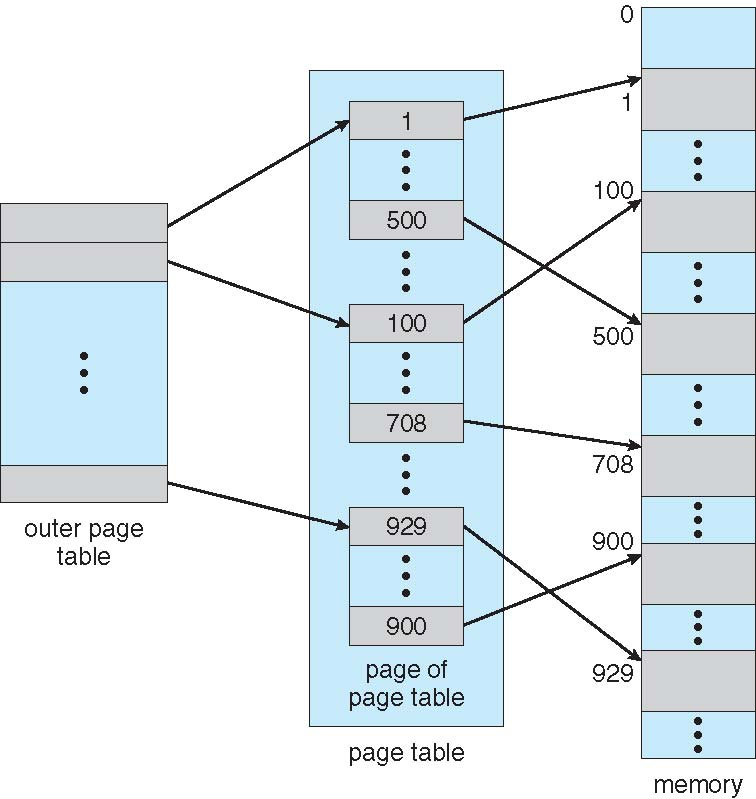
\includegraphics[width=0.7\textwidth]{page-table-3-hierarch}
			\caption{Diagram of a Hierarchical Page Table}
			\label{fig:paging:page-table-3-hierarch}
		\end{figure}
		&&& Diagram: See figure~\ref{fig:paging:page-table-3-hierarch}

		\begin{figure}[!htb]
			\centering
			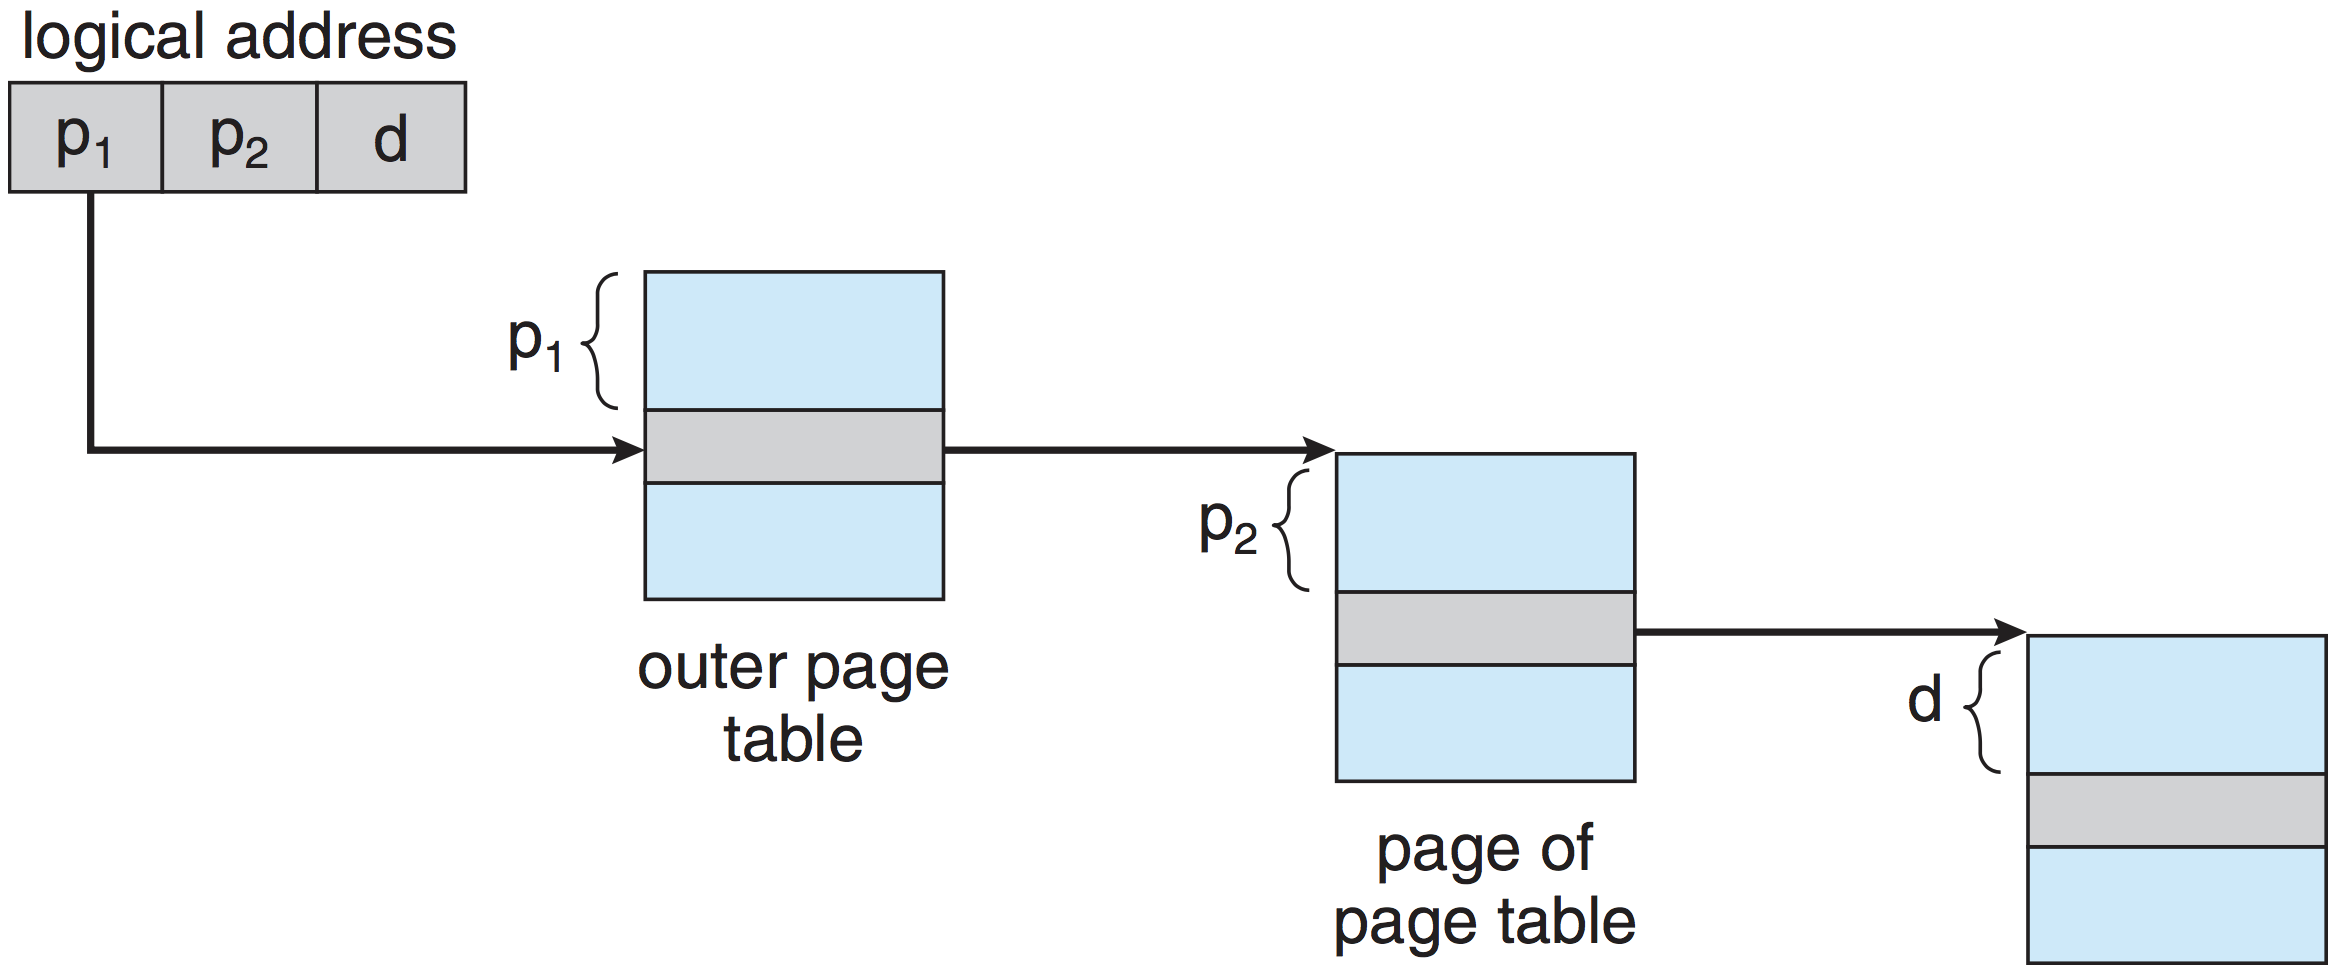
\includegraphics[width=0.7\textwidth]{page-table-4-hierarch-access}
			\caption{Accessing a Hierarchical Page Table}
			\label{fig:paging:page-table-4-hierarch-access}
		\end{figure}

	&& \textbf{Hashed page table:} Method to store page table entries non-contiguously by hashing page number to a linked list of elements, each with a page number and associated frame number
		&&& Diagram: See figure~\ref{fig:paging:page-table-6-inverted}

		\begin{figure}[!htb]
			\centering
			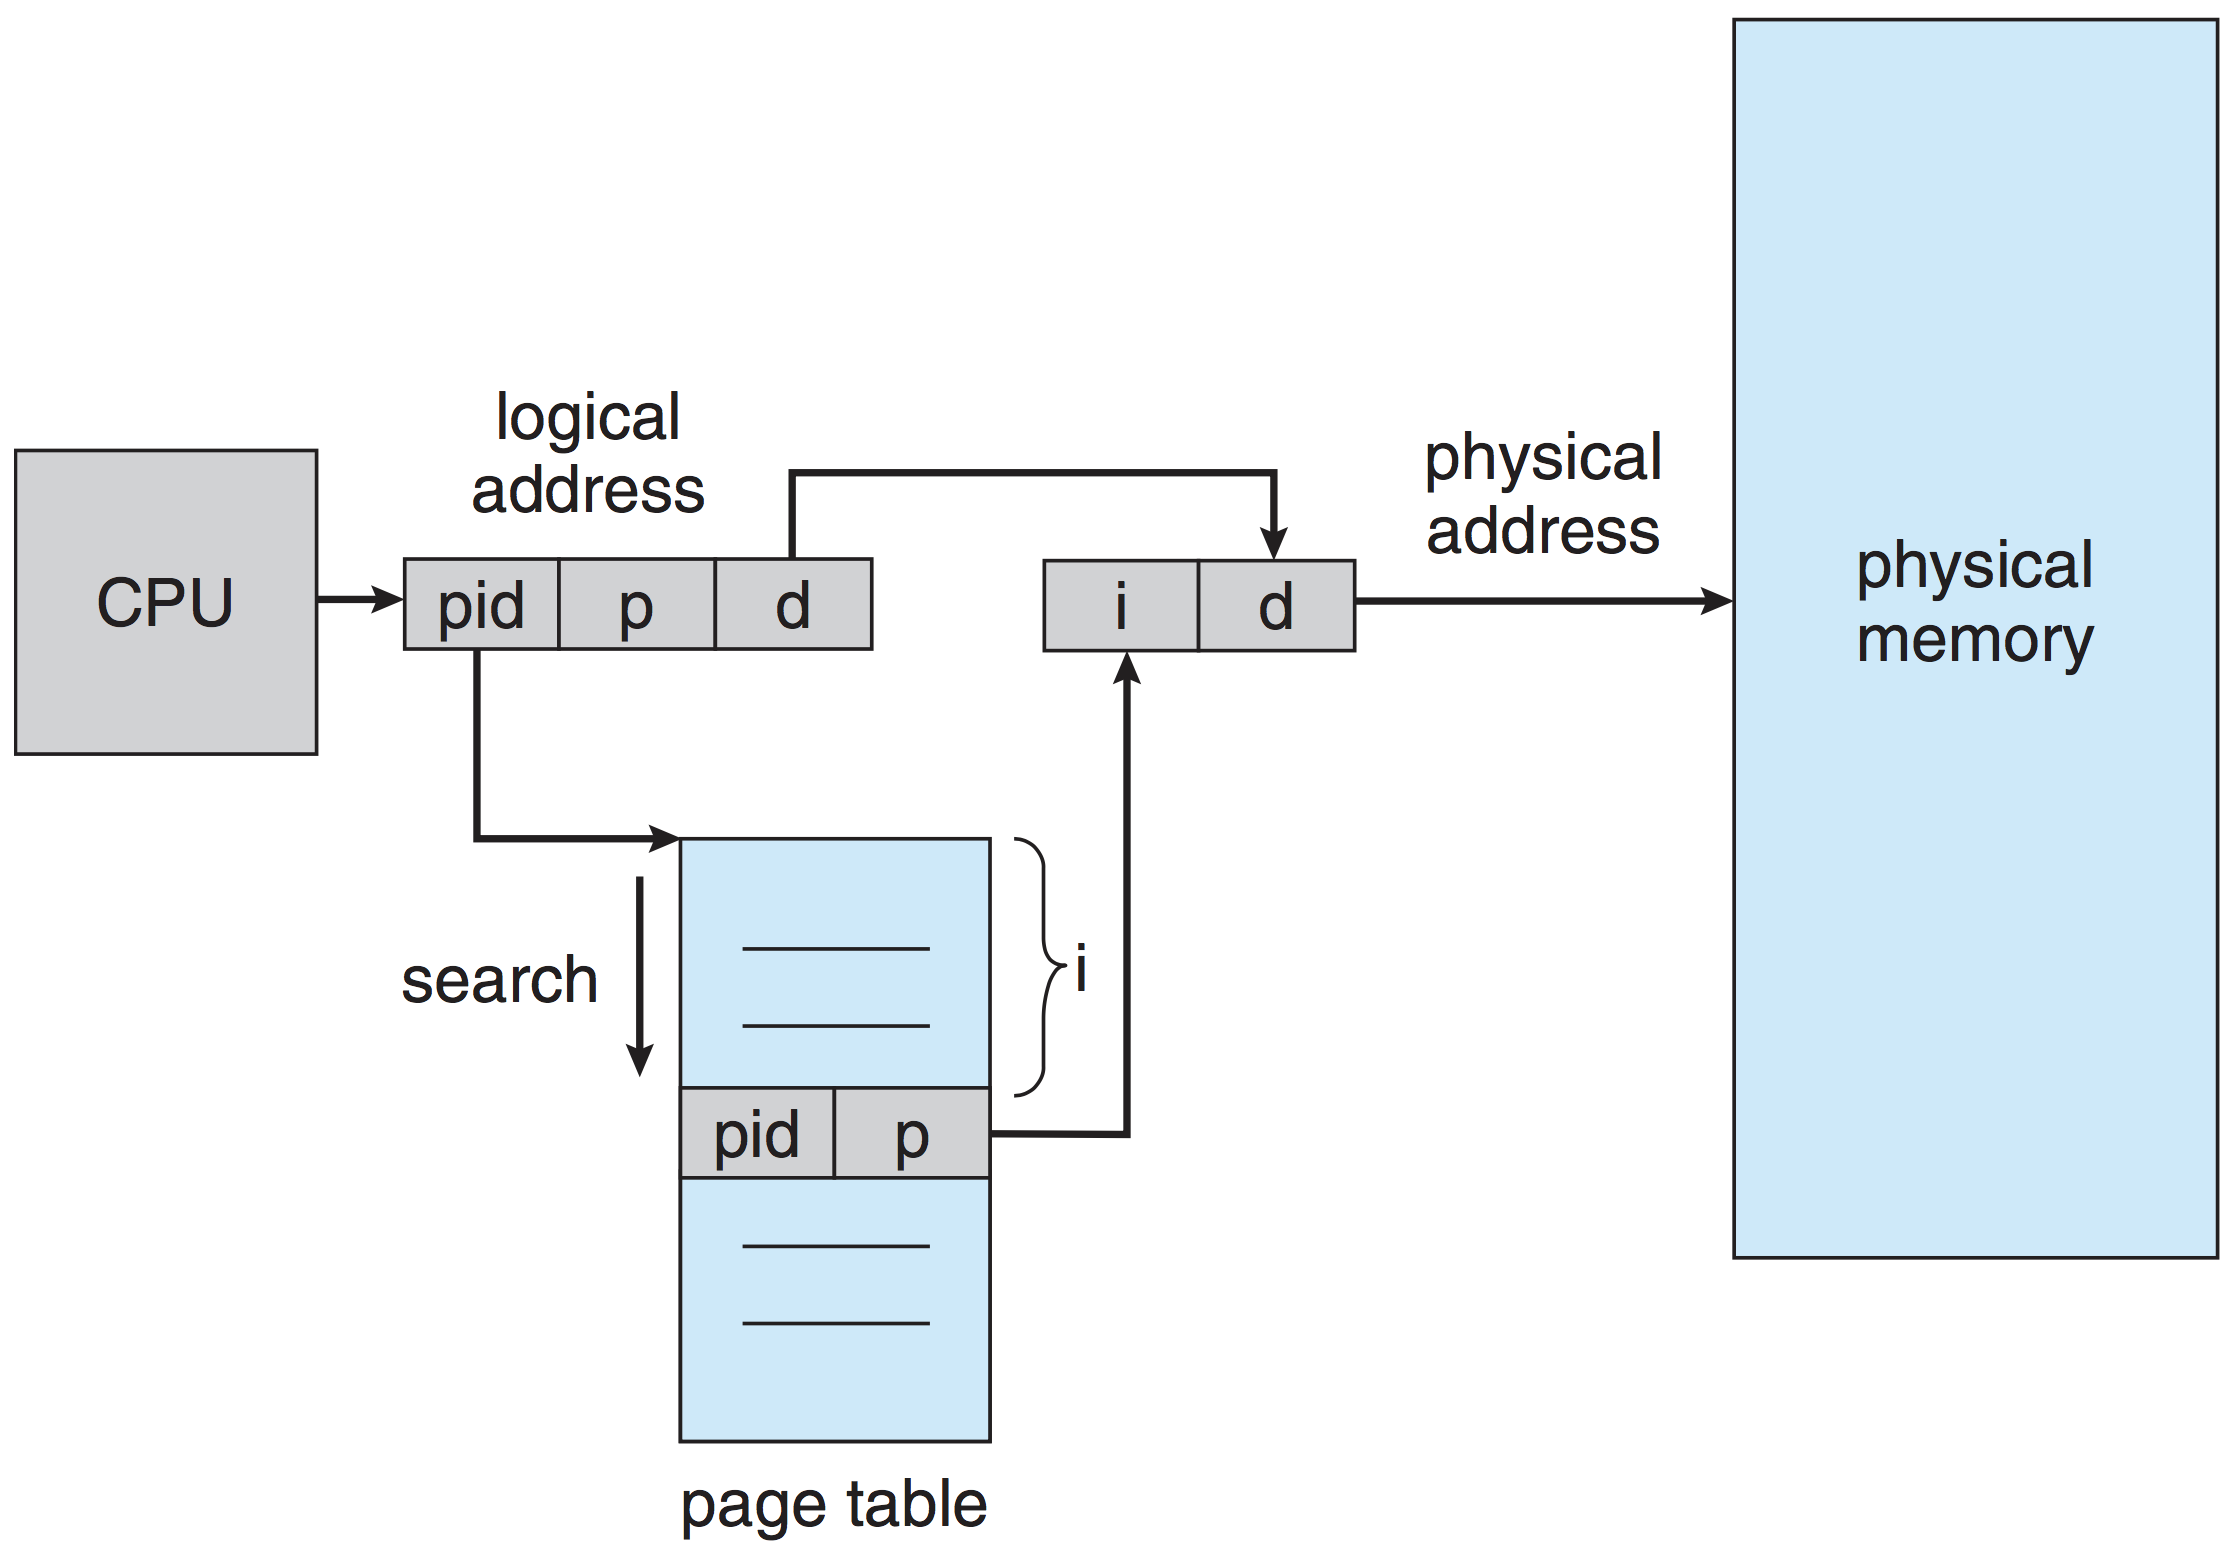
\includegraphics[width=0.7\textwidth]{page-table-6-inverted}
			\caption{Diagram of an Inverted Page Table}
			\label{fig:paging:page-table-6-inverted}
		\end{figure}
		
	&& \textbf{Inverted page table:} Method to use only one page table for all processes by using a table of page numbers (limited by amount of frames) and the process which owns the frame
		&&& Increases time to find a page reference
		&&& Creates difficulty in implementing a shared page

& \textbf{Internal fragmentation:} Situation where memory allocated as a fixed-size partition is larger than required which creates unusable excess memory

\end{easylist}
\subsection{Segmentation}
	\label{subsec:memory-management:segmentation}
\begin{easylist}

& \textbf{Segment:} Component of a program (e.g. function, object, main program)
	&& Segments are paged to avoid external fragmentation so the user interacts with the segments and the OS interacts with the pages

& \textbf{Segment table:} Structure which maps a logical address to a physical address using a base address and limit

\end{easylist}
\clearpage